% body3d: an anatomical muscle-activation viewer for the web, shaped by fat-free mass and tape measures.
% Build: latexmk -pdf body3d.tex   (figures are read from ../docs/images/, rendered by dev/figures.mjs)
\documentclass[10pt,twocolumn]{article}

\usepackage[a4paper,margin=18mm,columnsep=7mm]{geometry}
\usepackage[T1]{fontenc}
\usepackage[utf8]{inputenc}
\usepackage{lmodern}
\usepackage{microtype}
\usepackage{amsmath,amssymb}
\usepackage{graphicx}
\usepackage{booktabs}
\usepackage{tabularx}
\usepackage{xcolor}
\usepackage{tikz}
\usetikzlibrary{arrows.meta,positioning,fit,backgrounds,calc}
\usepackage[numbers,sort&compress]{natbib}
\usepackage[hidelinks]{hyperref}
\usepackage{caption}
\captionsetup{font=small,labelfont=bf}

\graphicspath{{../docs/images/}}
\newcommand{\eg}{e.g.\ }
\newcommand{\ie}{i.e.\ }
\newcommand{\vect}[1]{\mathbf{#1}}
\newcommand{\code}[1]{\texttt{#1}}

\title{\textbf{body3d}: An Anatomical Muscle-Activation Viewer for the Web,\\ Shaped by Fat-Free Mass and Tape Measures}
\author{Leonardo Marcos Gomes Salim}
\date{October 2026 --- version 0.2}

\begin{document}
\maketitle

\begin{abstract}
Fitness and rehabilitation applications tell people which muscles an exercise works, usually with
flat diagrams of a generic body. We present \textbf{body3d}, an open-source viewer that shows muscle
activation on an anatomical 3D body in a web page, and makes that body resemble the person. An
offline pipeline turns the BodyParts3D database into a rigged model of 135 muscles per side over a
full skeleton. A layered hypertrophy model grows the muscles without interpenetration; because it
is linear in the growth emphasis, splitting it by body region yields exactly additive morph targets
calibrated against the fat-free mass index (FFMI). A regularized least-squares fit then adjusts the
regions to a person's tape measures while conserving the muscle volume implied by their FFMI, with
a population prior learnt from the ANSUR~II anthropometric survey. On held-out people it predicts a
hidden limb girth with an RMS error of 1.5--1.6\,cm, against 3.3--3.7\,cm for the population mean:
as accurate as a ridge regression given only height, weight and body fat, but 0.2--0.3\,cm behind
it when every other tape is given --- the measured cost of explaining all tapes with one anatomical
body. Body composition in this evaluation is itself estimated from tapes. The viewer also chooses a
default camera for any activation set. Everything runs in three.js without decoders or WebAssembly,
at 2.3\,ms per frame on a desktop GPU and about 10\,ms per fit.
\end{abstract}

\section{Introduction}

``Which muscles does this exercise work?'' is among the most common questions in strength training,
and applications answer it with a highlighted silhouette. Two shortcomings of that answer motivated
this work. First, a 2D map hides depth and side: the triceps is behind the arm, the gluteus medius
sits above and lateral to the maximus, the brachialis lies under the biceps. Second, the body shown
is nobody in particular, while the same applications store the person's weight, body fat and girths.

body3d is a web component that addresses both: an anatomical body of individually named muscles
over a skeleton, coloured by activation, that can be orbited, tapped and posed, and whose shape
follows the person's fat-free mass and tape measures. It must run in ordinary web pages --- on
phones, inside applications with strict Content-Security-Policies that forbid WebAssembly and
\code{eval} --- and must be embeddable as a library, a custom element or an iframe.

Our contributions are:
\begin{itemize}\itemsep1pt
\item a reproducible pipeline from the BodyParts3D anatomical database to a rigged, quantized glTF
  model, including the synthesis of a missing muscle by elastic fibres draped over a distance field
  (Section~\ref{sec:model});
\item a layered hypertrophy model whose region-wise split is \emph{exactly additive}, giving 14 morph
  targets calibrated against fat-free mass (Section~\ref{sec:hypertrophy});
\item a tape-measure fit that reconciles regional girths with total muscle mass, with closed-form
  girth and volume models, a population prior calibrated on ANSUR~II and robust outlier handling,
  evaluated out of sample against statistical baselines (Sections~\ref{sec:fit} and~\ref{sec:eval});
\item an automatic choice of the camera for an activation set, from per-group visibility in a
  picking buffer (Section~\ref{sec:views});
\item a runtime design for the web: per-part state in a data texture, dual-quaternion skinning on
  quantized geometry, GPU picking and on-demand rendering (Section~\ref{sec:runtime}).
\end{itemize}
We also report what the evaluation could not settle --- real left--right asymmetry, a trained
population, agreement with coaches on views --- and release the protocols and scripts for those
studies.

\section{Related work}

\paragraph{Anatomical data.}
BodyParts3D~\cite{mitsuhashi2009bodyparts3d} maps concepts of the Foundational Model of
Anatomy~\cite{rosse2003fma} to polygon meshes of one adult male body; since 2025 it is distributed
under CC~BY~4.0. It is, to our knowledge, the only open dataset with volumetric, individually named
muscles tied to an ontology. Statistical body models such as SMPL~\cite{loper2015smpl} describe the
skin surface only; musculoskeletal simulators such as OpenSim~\cite{delp2007opensim} represent
muscles as lines of action.

\paragraph{Anatomical body modelling.}
Graphics research has built detailed, simulated musculature: Teran et al.~\cite{teran2005muscle}
extracted and simulated muscles from the Visible Human data; Lee et
al.~\cite{lee2009upperbody} modelled and controlled the upper body with hundreds of muscles; Saito
et al.~\cite{saito2015bodybuilding} grew muscle and fat with physics-based growth and elasticity to
produce a range of body shapes from one anatomical template; Kadle\v{c}ek et
al.~\cite{kadlecek2016anatomy} fitted a template anatomy to 3D surface scans. These methods solve
volumetric elasticity problems offline or near-interactively and take scans as input.

\paragraph{The inside from the outside.}
A line of learned models infers internal anatomy from the body surface of SMPL.
OSSO~\cite{keller2022osso} predicts the skeleton from the skin, trained on paired DXA scans;
SKEL~\cite{keller2023skel} re-rigs SMPL with a biomechanically accurate skeleton.
HIT~\cite{keller2024hit}, the closest to our goal, learns from segmented MRI registered to SMPL an
implicit model of where subcutaneous fat, lean tissue (muscles and organs together) and long bones
lie inside a body of given shape and pose. body3d differs in what it models and from what: named
individual muscles rather than tissue classes, inferred from the tape measures and body composition
people record rather than a surface scan, by a small calibrated optimization rather than a learned
network, and evaluated by a GPU in a web page.

\paragraph{Bodies from measurements.}
Synthesizing a body from anthropometric measurements is an old problem for skin surfaces. Seo and
Magnenat-Thalmann~\cite{seo2003sizing} learnt from range scans an interpolation from sizing
parameters to body shape; Wuhrer and Shu~\cite{wuhrer2013measurements} estimated shapes from
CAESAR-type measurements with a statistical shape model and a nonlinear optimization that
extrapolates beyond the training set; Anny~\cite{bregier2025anny}, an open parametric model, spans
ages and body types through semantic phenotype parameters calibrated on WHO statistics. body3d
solves the analogous problem one layer down: the musculature behind given girths, with a prior on
muscle per region.

\paragraph{Body composition and anthropometry.}
The fat-free mass index (FFMI) normalized by height~\cite{kouri1995ffmi,schutz2002ffmi} measures
muscularity independently of fat; skeletal muscle mass relates to fat-free mass through whole-body
MRI studies~\cite{janssen2000smm,midorikawa2007athletes,abe2018upperlimit}, and corrected girths
(girth minus $\pi$ times the skinfold)~\cite{heymsfield1982arm,lee2000anthropometric} relate tapes to
muscle cross-sections. The US Navy method~\cite{hodgdon1984navy} estimates body fat from girths.
ANSUR~II~\cite{gordon2014ansur} provides 93 measurements on 6\,068 U.S. Army personnel.

\section{System overview}

\begin{figure}[t]
\centering
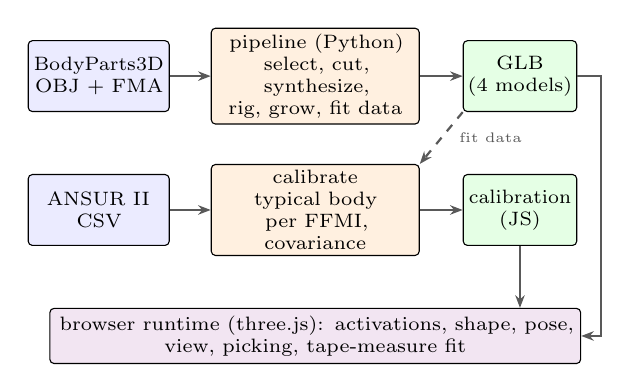
\begin{tikzpicture}[x=1mm,y=1mm, every node/.style={font=\scriptsize},
  box/.style={draw, rounded corners=1.5pt, align=center, inner sep=2pt, minimum height=9mm},
  ar/.style={-{Stealth[length=1.6mm]}, thick, gray!70!black}]
\node[box, fill=blue!8, text width=16.5mm] (bp) at (-1.5,0) {BodyParts3D\\OBJ + FMA};
\node[box, fill=orange!12, text width=25mm] (pipe) at (26,0) {pipeline (Python)\\select, cut, synthesize,\\rig, grow, fit data};
\node[box, fill=green!10, text width=13mm] (glb) at (52,0) {GLB\\(4 models)};
\node[box, fill=blue!8, text width=16.5mm] (ansur) at (-1.5,-17) {ANSUR II\\CSV};
\node[box, fill=orange!12, text width=25mm] (cal) at (26,-17) {calibrate\\typical body per FFMI,\\covariance};
\node[box, fill=green!10, text width=13mm] (calj) at (52,-17) {calibration\\(JS)};
\node[box, fill=violet!10, text width=66mm, minimum height=7mm] (rt) at (26,-33) {browser runtime (three.js): activations, shape, pose,\\view, picking, tape-measure fit};
\draw[ar] (bp) -- (pipe);
\draw[ar] (pipe) -- (glb);
\draw[ar] (ansur) -- (cal);
\draw[ar] (cal) -- (calj);
\draw[ar] (calj) -- (calj |- rt.north);
\draw[ar] (glb.east) -- ++(3,0) |- (rt.east);
\draw[ar, dashed] (glb.south west) -- node[right, xshift=1mm, font=\tiny] {fit data} (cal.north east);
\end{tikzpicture}
\caption{Offline pipeline and runtime. The calibration is computed on the exported model's fit data
and keyed by its fingerprint.}
\label{fig:overview}
\end{figure}

Everything expensive happens offline (Fig.~\ref{fig:overview}): mesh selection and cleaning,
synthesis, joint placement, skinning weights, hypertrophy morphs, baked ambient occlusion and the
data of the tape fit. The browser receives a self-describing glTF file~\cite{khronos2017gltf} per
model (male and female, each at two resolutions: 380\,k and 159\,k triangles) and performs only what
reacts to the person. The calibration is computed by a separate step on the exported fit data;
because it depends on the exact geometry, it is keyed by a hash of those data, and a rebuilt model
without a matching calibration fails the test suite. The pipeline is deterministic: a rebuild from
the same sources produces byte-identical geometry.

\section{Building the anatomical model}\label{sec:model}

\paragraph{Selection.}
Of the 2\,234 BodyParts3D meshes (426 muscles, 225 bones, 30 cartilages), an explicit table lists
133 muscles per side by concept name, three connective tissues, rules assigning bones to 52 rig
segments, and the viscera used later as a hypertrophy core; with the two structures added below ---
the synthesized latissimus dorsi and the rectus abdominis cut out of the abdominal wall --- the model
has 135 muscles per side. Table-driven selection replaced name-based heuristics after two failures:
a pattern meant for foot bones matched a laryngeal cartilage, and one file named ``left'' lies in
the right hand. The build stops on any inconsistency (missing names, a part with pieces on both
sides, a bone far from its segment).

\paragraph{Vocabularies.}
Muscles belong to 44 anatomical groups (\eg the three parts of the pectoralis and of the deltoid,
gastrocnemius separate from soleus), labelled in English and Brazilian Portuguese. A 25-group
training vocabulary (``Chest'', ``Lats'', ``Upper Back'') maps onto groups with weights, \eg
``Brachialis'' activates the brachialis at 1 and the brachioradialis at 0.5. Names resolve
case- and accent-insensitively with a fixed precedence.

\paragraph{Cut and synthesized structures.}
In BodyParts3D the external-oblique mesh is the whole anterior abdominal wall. We cut the rectus
abdominis out along the linea semilunaris, measured as a groove on horizontal slices (5\,cm from
the midline near the pubis, 6.3--7\,cm at the navel, 9\,cm at the costal margin), by splitting
triangles on the zero set of a scalar field so both parts stay glued.

The database has no latissimus dorsi. We synthesize it as $K=36$ fibres from a fleshy origin
measured on this body (spinous processes under the trapezius, the lateral border of the erectors,
the iliac crest) to the intertubercular sulcus of the humerus. Let $D$ be the signed distance to a
\emph{support} --- ribs, spine, scapula, pelvis, deep muscles and viscera, closed morphologically
and filled slice by slice so no fibre crosses the thorax. Each fibre $\{\vect p_i\}$ starts as an
arc around the trunk and alternates a shortening step and a projection:
\begin{align}
\vect p_i &\leftarrow \vect p_i + \tfrac12\big(\tfrac12(\vect p_{i-1}+\vect p_{i+1})-\vect p_i\big),\\
\vect p_i &\leftarrow \vect p_i + \max\big(0,\delta - D(\vect p_i)\big)\,\nabla D/\|\nabla D\|,
\end{align}
until it lies taut over the support (multiresolution: 9, 17, 33, 65, 96 points). The sheet of
fibres receives a thickness by volume conservation --- proportional to the width at the origin over
the local width, capped at 2\,cm --- tapering at the free borders and into a flat tendon (Fig.~\ref{fig:synth}).
The thoracolumbar aponeurosis is deliberately not drawn: it would hide the erectors, which are
activated in many exercises.

\begin{figure}[t]
\centering
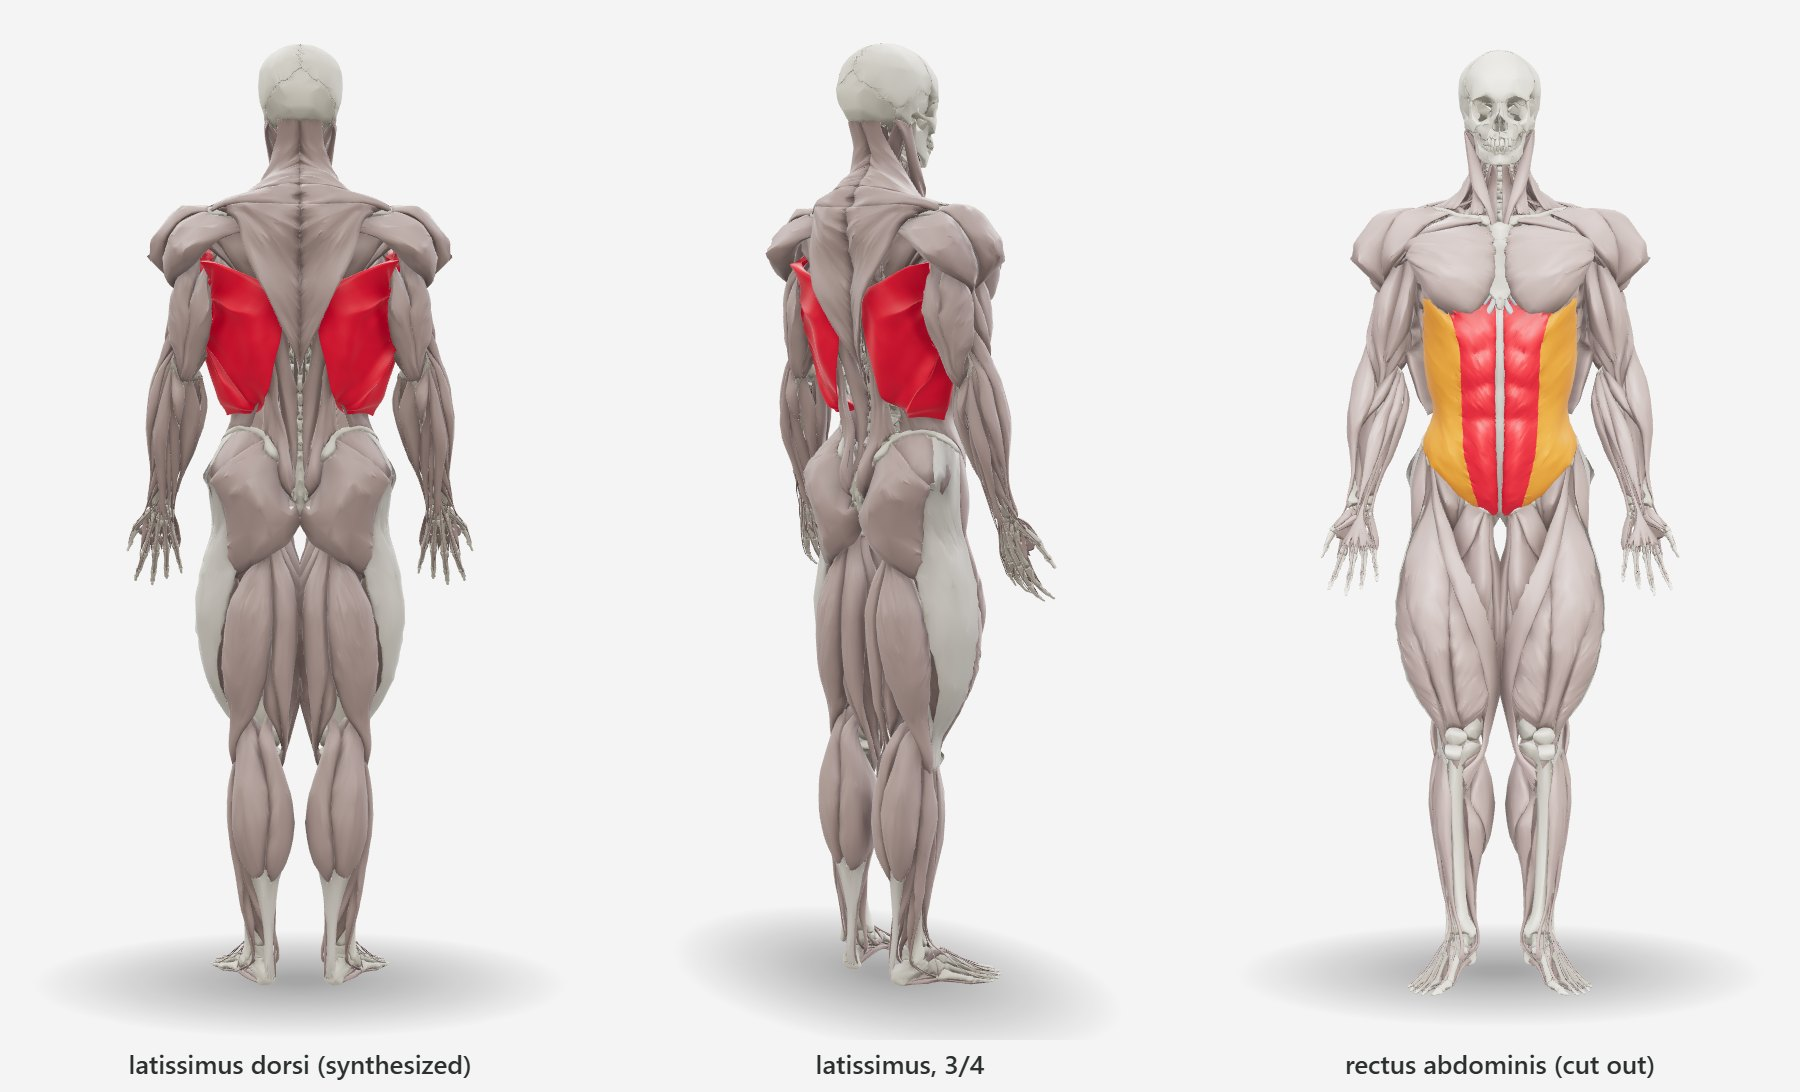
\includegraphics[width=\columnwidth]{synthesized.jpg}
\caption{The synthesized latissimus dorsi (left, centre) and the rectus abdominis cut out of the
abdominal wall (right).}
\label{fig:synth}
\end{figure}

\paragraph{Geometry.}
Meshes are welded, decimated by quadric error~\cite{garland1997qem} to a budget spread by surface
area, and smoothed by Taubin's $\lambda|\mu$ filter~\cite{taubin1995fair} with fixed borders, which
does not shrink and is linear. Volumetric operations use a voxelization by ray parity along three
axes with a majority vote, robust to the database's non-watertight meshes (a flood fill inflated
the left thigh, whose femur leaks on the grid).

\paragraph{Rig and weights.}
Fifty-two joints have identity rotation in the rest pose and are placed from bone geometry:
least-squares spheres on the femoral and humeral heads, the midpoints of epicondyles and malleoli,
the centres of intervertebral disks, and bone contacts for wrists and fingers. Skinning weights are
inverse cubed distances to bone surfaces, restricted to the segments that dominate a part and their
chain neighbours, with the dominant segment weighted 4$\times$; without these rules a hand hanging
by the thigh followed the leg, and the biceps stretched across the elbow.

\paragraph{Female proportions.}
BodyParts3D has one male body. The female model applies per-segment affine transforms through the
skinning weights (pelvis width $\times$1.14, thorax $\times$0.92, clavicles $\times$0.88, +4$^\circ$
carrying angle, knee valgus, smaller hands, feet and neck) before the hypertrophy, followed by a
female distribution of muscle gain.

\section{Layered hypertrophy}\label{sec:hypertrophy}

\paragraph{From FFMI to muscle volume.}
Body size is expressed by the normalized FFMI~\cite{kouri1995ffmi},
\begin{equation}
F = \frac{\mathrm{FFM}}{h^2} + 6.1\,(1.8 - h),
\end{equation}
with fat-free mass FFM in kg and height $h$ in metres. Skeletal muscle mass is
$\mathrm{SMM}=k(F)\,\mathrm{FFM}$. Whole-body MRI puts SMM at 38\,\% and 31\,\% of body mass in men and
women~\cite{janssen2000smm}, which with the body fat of those samples gives $k\approx0.49$ and $0.47$.
The ratio is higher in trained people --- 0.477 against 0.447 in college athletes and
non-athletes~\cite{midorikawa2007athletes}, about 8\,\% higher in very large
athletes~\cite{abe2018upperlimit} --- so $k$ rises linearly to 0.56 at $F=26$ for men (0.52 at 22 for
women). The direction is documented; the slope, about twice the reported differences, is our
assumption. Its reach is limited: after the calibration of Section~\ref{sec:fit} it only sets the
trunk of the typical body, and half the slope would make the default male's shoulders 2.7\,cm
narrower. The represented muscle volume is $V = c\,\mathrm{SMM}/\rho$ with $\rho = 1.06$\,kg/L and a
coverage $c = 0.92$ for the deep muscles the model lacks. The base body is 1.707\,m tall with
18.7\,L of muscle, $F \approx 15$; at the default $F = 26$ the male model carries 39.6\,L.

\paragraph{The stacking integral.}
Inflating each muscle along its normals makes layers cross. Instead, let $\tilde D$ be the smoothed
distance to the \emph{core} (bones, cartilage and viscera), $\vect u = \nabla \tilde D/\|\nabla\tilde D\|$
and $e(\vect x)$ the growth emphasis of the muscle at $\vect x$ (zero outside muscle). A surface point
moves by
\begin{equation}
\vect d(\vect p) = g\,\vect u(\vect p) \int_0^{\ell(\vect p)} e\big(\vect p - s\,\vect u(\vect p)\big)\,ds,
\label{eq:stack}
\end{equation}
the thickening of all muscle between the point and the core, with $\ell$ bounded by 1.3 times the
true distance to the core. The inner face of a muscle moves with the outer face of the one below, so
layers remain stacked by construction; in the abdomen the core is the viscera, so the wall thickens
without the belly inflating. The global gain $g$ is solved so that the muscle volume meets the
target; the emphasis (\eg lateral deltoid 1.65, obliques 0.6 for men; gluteus maximus 1.6 for
women) distributes the gain like a trained physique.

\paragraph{Exactly additive regional morphs.}
Partition the muscle groups into $R=14$ regions (upper arm, forearm, thigh and lower leg per side;
shoulders, chest, back, neck, core, hips) and write $e = \sum_r e_r$. Eq.~\eqref{eq:stack} is linear in
$e$, and every later step --- the isotropic limbs below, vector smoothing over the mesh, Taubin
smoothing with fixed borders, the uniform scale to the target height --- is linear in the
displacements. Therefore the per-region displacements $\vect m_r$ obtained from $e_r$ satisfy,
exactly,
\begin{equation}
\vect x(\vect w) = \vect x_0 + \sum_{r=1}^{R} w_r\,\vect m_r,
\end{equation}
and $w_r = t$ for all $r$ reproduces the uniform body at gain $t$. The pipeline checks the sum on
every vertex (the largest difference is $1.5\times10^{-15}$\,m, float64 rounding) and exports
$\vect x_0$ at the minimum of the FFMI range and the $\vect m_r$ as glTF morph targets, with a table
from $F$ to the uniform weight (Fig.~\ref{fig:ffmi}).

\begin{figure}[t]
\centering
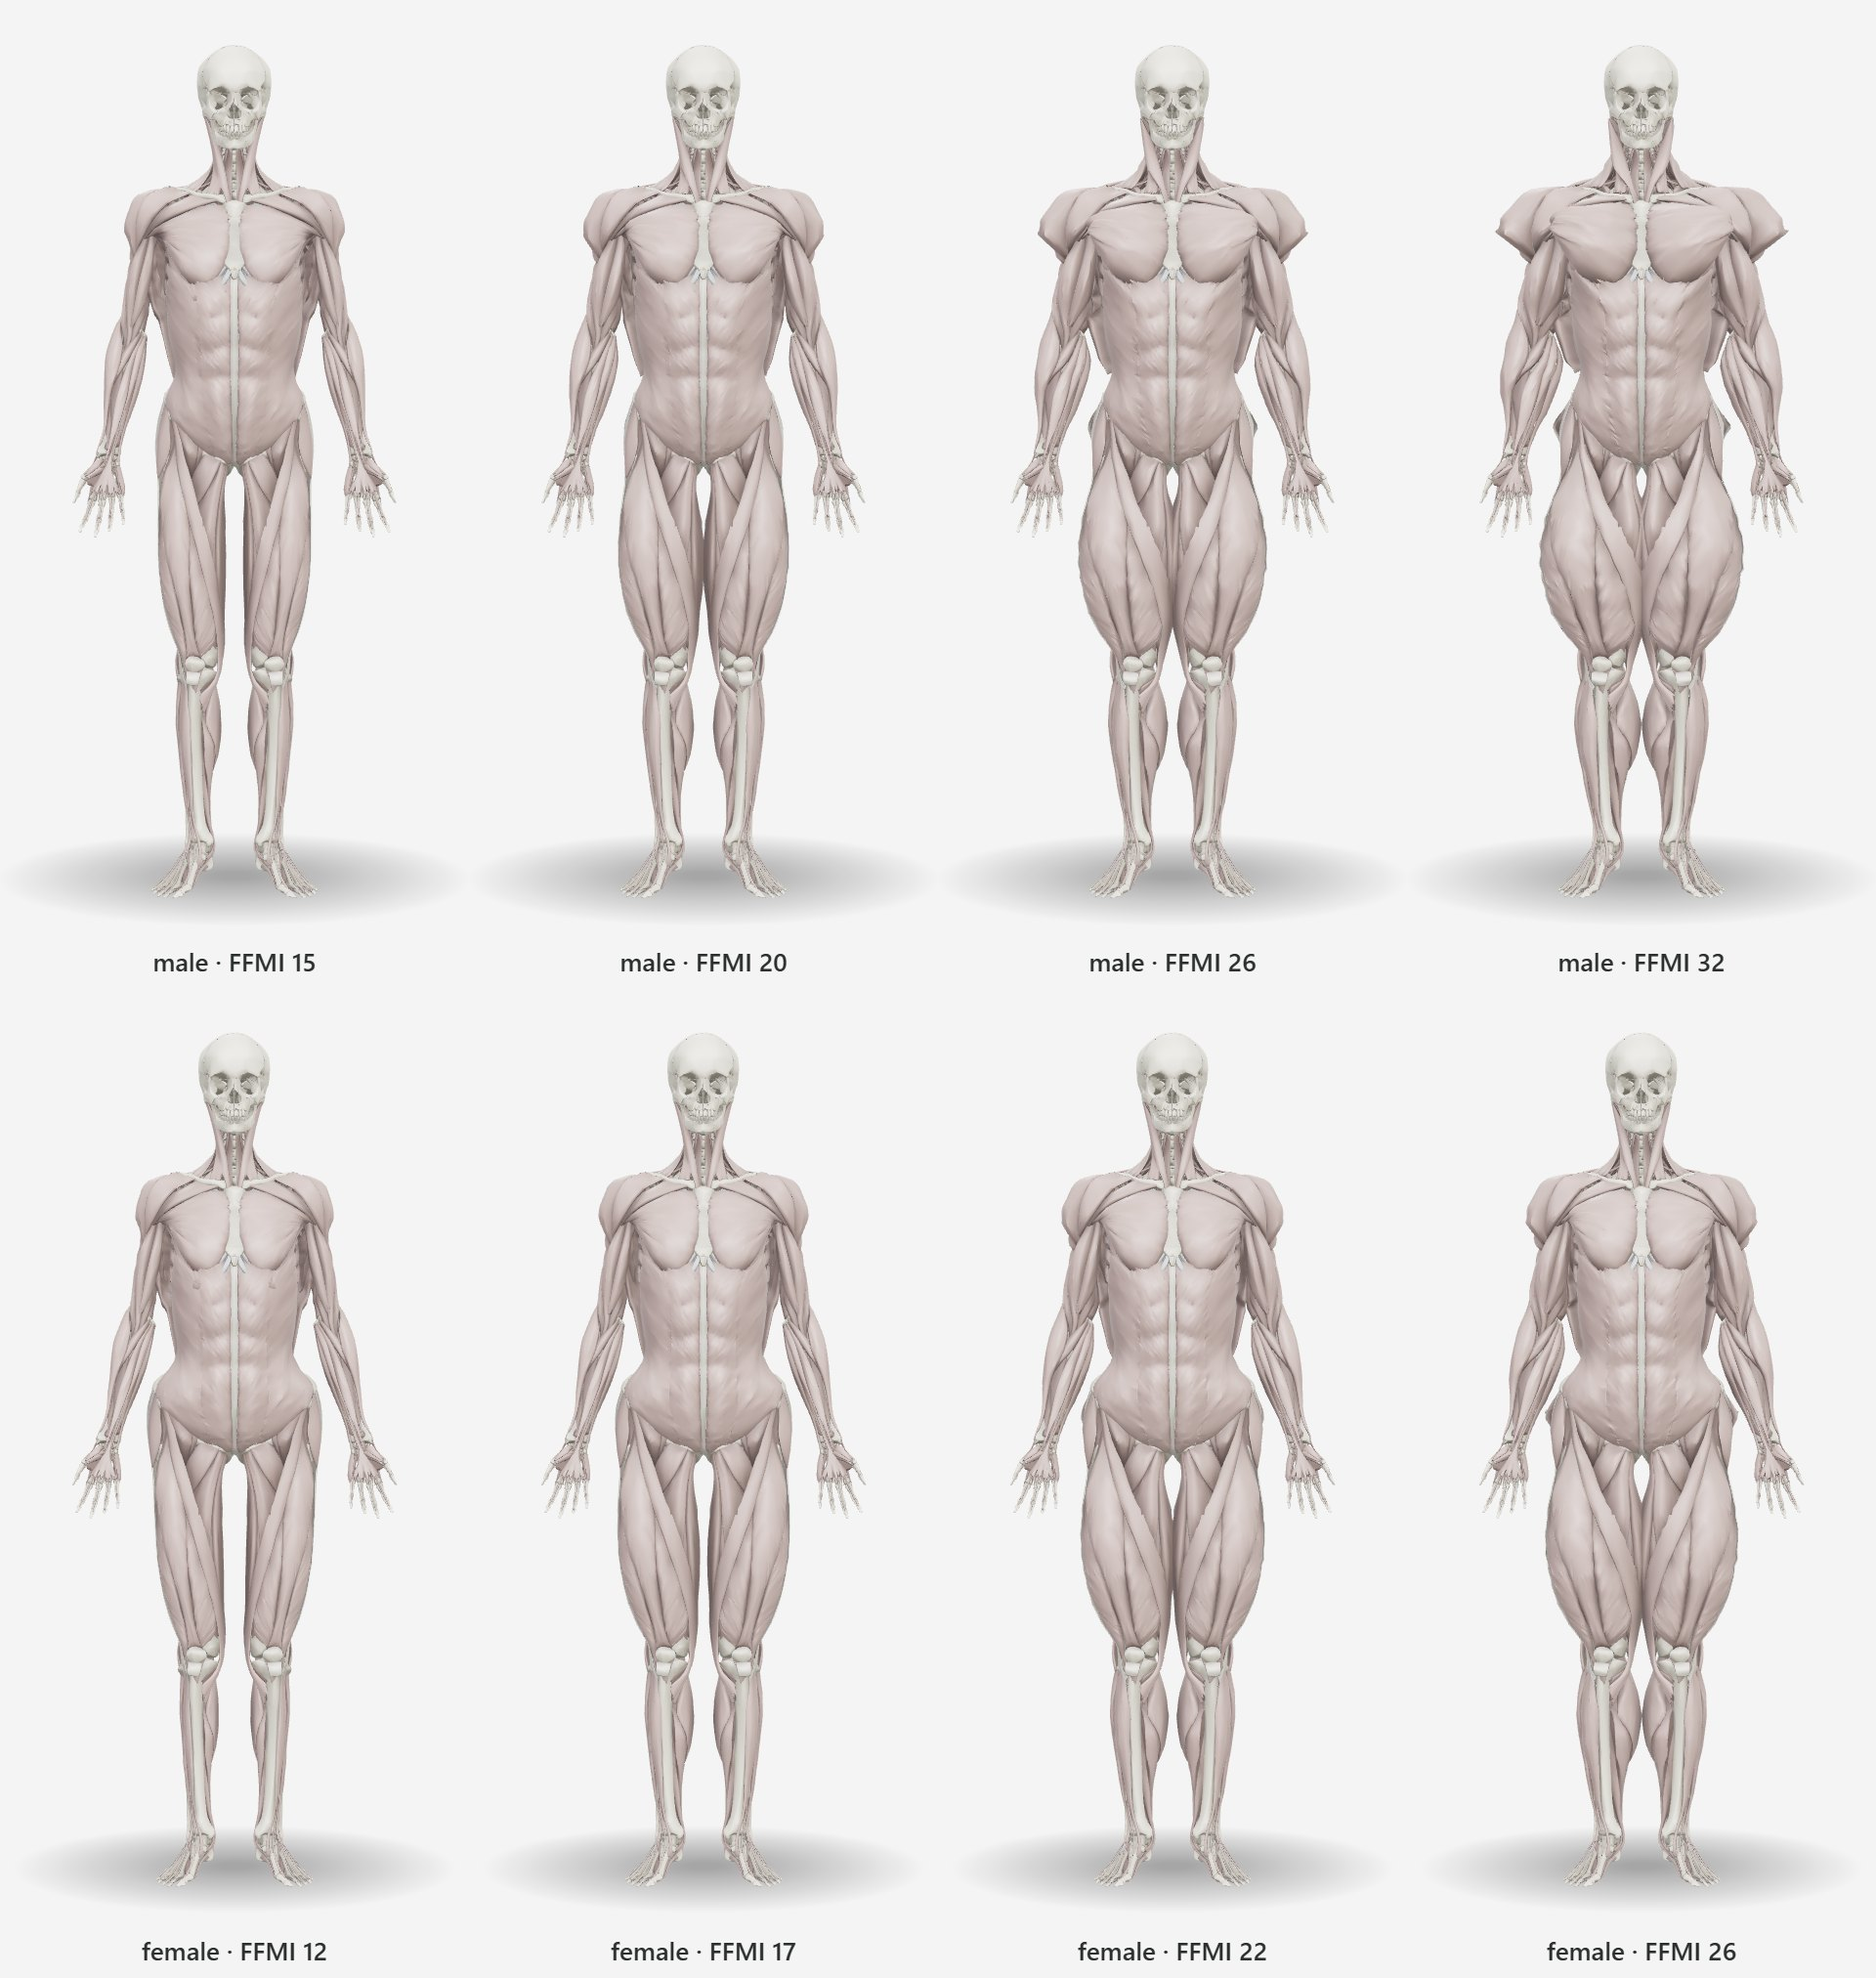
\includegraphics[width=\columnwidth]{ffmi-range.jpg}
\caption{The male model at FFMI 15, 20, 26 and 32 and the female model at 12, 17, 22 and 26 (typical
bodies, Section~\ref{sec:fit}).}
\label{fig:ffmi}
\end{figure}

\paragraph{Isotropic limbs.}
Stacking thickens a layer along the thickness it already has; the arm, whose biceps and triceps are
thick antero-posteriorly, grew almost only in depth (a $10\times21$\,cm section at $F=26$). Mid-limb,
we replace the displacement by a radial scale about each section's centre, blended in by limb and
faded near the joints. The scale of a level, $s=\sqrt{1+P\bar m/A}$ for a hull of area $A$,
perimeter $P$ and mean outward displacement $\bar m$, is computed \emph{once}, from the stacking
displacement per unit gain on the rest shape, and enters as a fixed field: the hypertrophy stays
linear and the morphs exactly additive. It matches the outline area that stacking adds at unit gain
only to first order, and does not conserve each level's volume. Measured against plain stacking over
the drawable range, a limb's own muscle volume changes by $-9$ to $+23$\,\% and its mid-limb outline
area by $-14$ to $+18$\,\%, and the upper arm's field enlarges the latissimus near the axilla, which
stacking would only have translated. The FFMI table is computed after this step, on the measured
volume, so the drawn FFMI stays calibrated; over the whole body the limbs' share of the uniform
growth moves from 68.7 to 69.4\,\% (male).

\section{Runtime}\label{sec:runtime}

\paragraph{Format.}
Positions are int16 and normals int8 (KHR\_mesh\_quantization), skin weights and ambient occlusion
uint8, indices uint16; three.js~\cite{threejs} reads them natively, so no decoder, worker or
WebAssembly is needed. One quantization box covers the body and its dequantization is folded into
the inverse bind matrices, so a single skin serves all meshes. Soft tissue is split into 14 meshes
by dominant region, each carrying only the 1--10 morph targets that move it; three quarters of the
targets are sparse. The full models are 11\,MB (5.7\,MB gzipped), the lite ones 5\,MB (2.6\,MB).

\paragraph{Shading.}
All per-part state (activation, highlight, dimming, kind) lives in a $1\times547$ RGBA data texture
indexed by a per-vertex part attribute: changing what is active rewrites at most 2.2\,kB, and the body
remains 15 draw calls. The material is three.js's physically based material with replaced shader
chunks: an activation colour ramp, a rim term, baked ambient occlusion, and \emph{dual-quaternion
skinning}~\cite{kavan2008dqs}, which preserves volume under the twists of the bodybuilding poses
where linear blending collapses shoulders and elbows. Because the bone matrices carry the uniform
dequantization scale, the shader extracts it from the first column before converting the rotation
to a quaternion and reapplies it before the rigid part.

\paragraph{Picking and rendering.}
A tap renders a $1\times1$ off-screen pass in which every fragment writes its part index; the answer
is exact on the skinned, morphed, posed body at the cost of one pixel (1.1\,ms on a desktop GPU),
without a CPU copy of deformed geometry. The render loop draws only after a change. Six classic
poses per sex are rotation lists about body axes, grounded by lowering the body until the lowest
foot sample touches the floor (Fig.~\ref{fig:poses}).

\begin{figure*}[t]
\centering
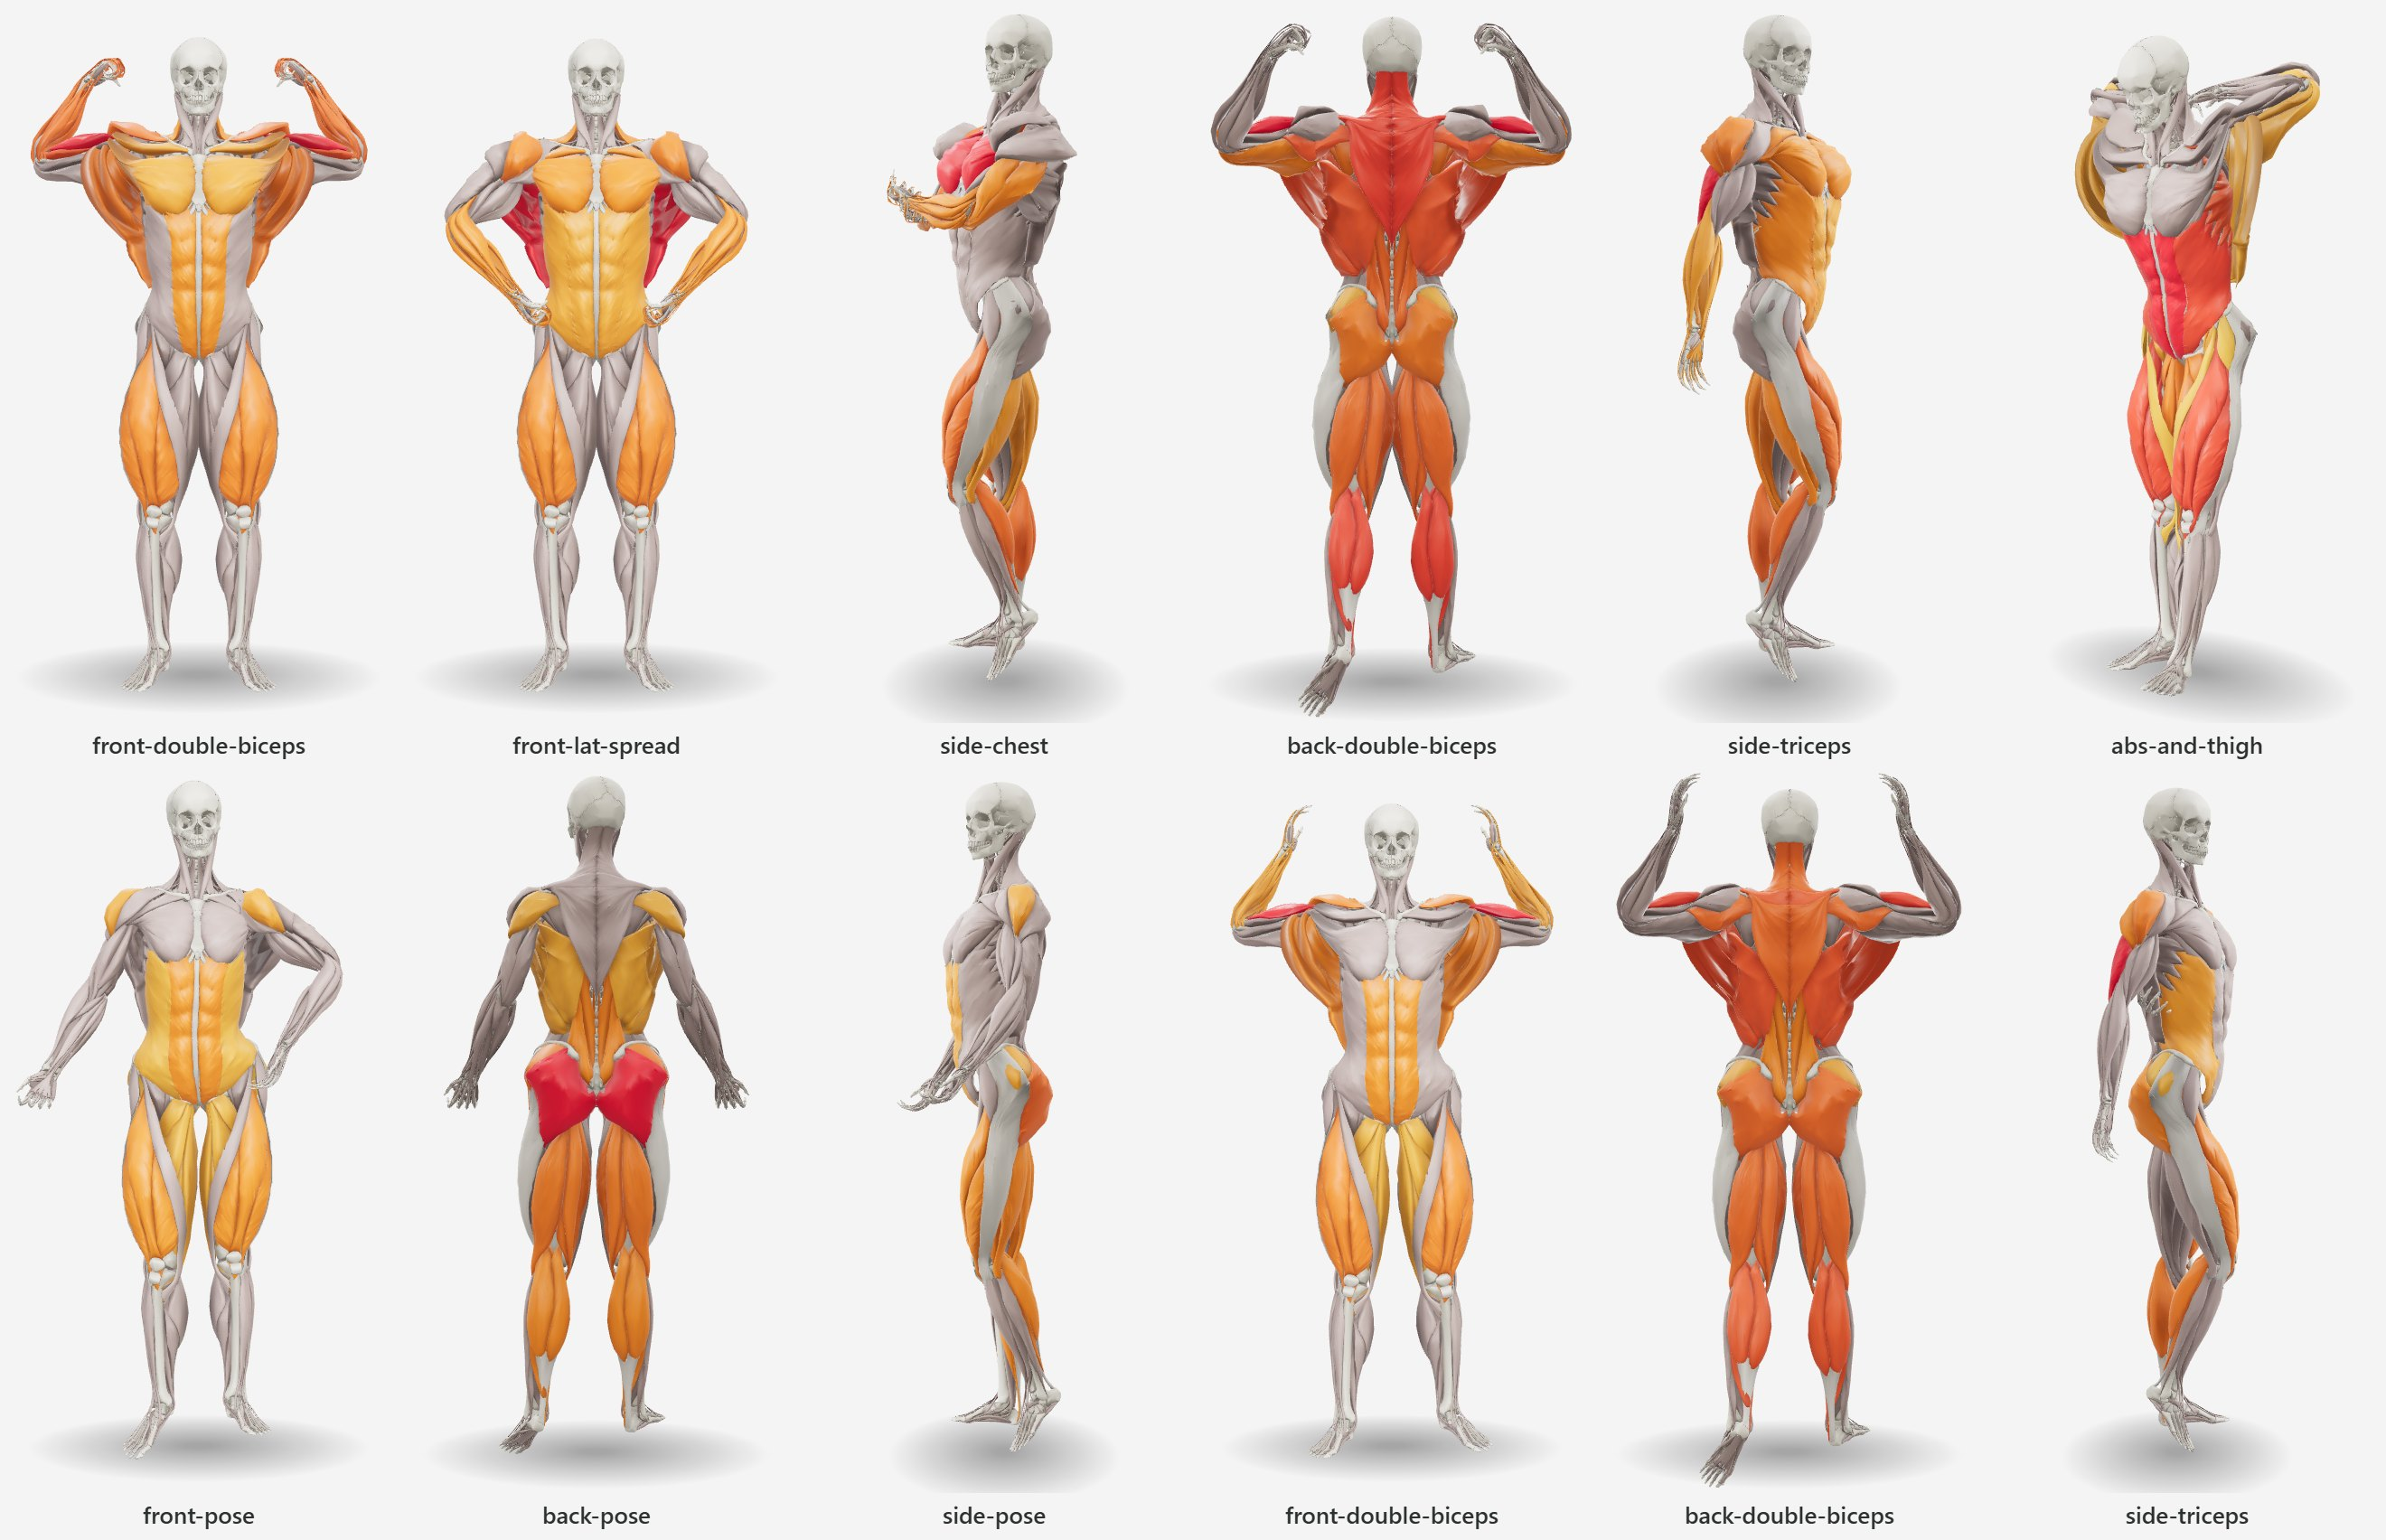
\includegraphics[width=\textwidth]{poses.jpg}
\caption{Six poses per model, each with the activations it suggests, rendered with dual-quaternion skinning.}
\label{fig:poses}
\end{figure*}

\section{Choosing a view}\label{sec:views}

A view is stored relative to the body as yaw, pitch, zoom and a focus point in body heights, so it
fits either model, any FFMI and any viewport. For an activation set $a_i$ on parts $i$, let groups
$\mathcal{G}$ have weights $\omega_g=\max_{i\in g} a_i^2$. We render the picking pass at $90\times150$
pixels from eight azimuths (front, back, sides, the four 3/4 views) at pitches $4.6^\circ$ and
$16^\circ$, count the pixels $n_g(v)$ of each group in each view $v$, and score
\begin{equation}
S(v) = \beta(v)\sum_{g\in\mathcal G}\omega_g\,\frac{n_g(v)}{\max_{v'} n_g(v')},
\end{equation}
with $\beta=1.10$ for the front, $1.07$ for the back and $0.94$ for the raised camera. Normalizing per
group makes a group count by how well a view shows it relative to its best view, not by its size:
with raw pixel counts the large trapezius out-voted the lateral deltoid and lateral raises were
shown from behind. Squaring the activation lets secondary muscles break ties only. In the winning
view, the bounding box of the key muscles (weight $\geq\frac12\max\omega$) sets a zoom of
$1/(1.6\max(b_w,b_h))$, capped at $1.5$, and a focus at its centre, unless the box spans more than
62\,\% of the height. The computation takes 23\,ms on a desktop GPU.

\begin{figure*}[t]
\centering
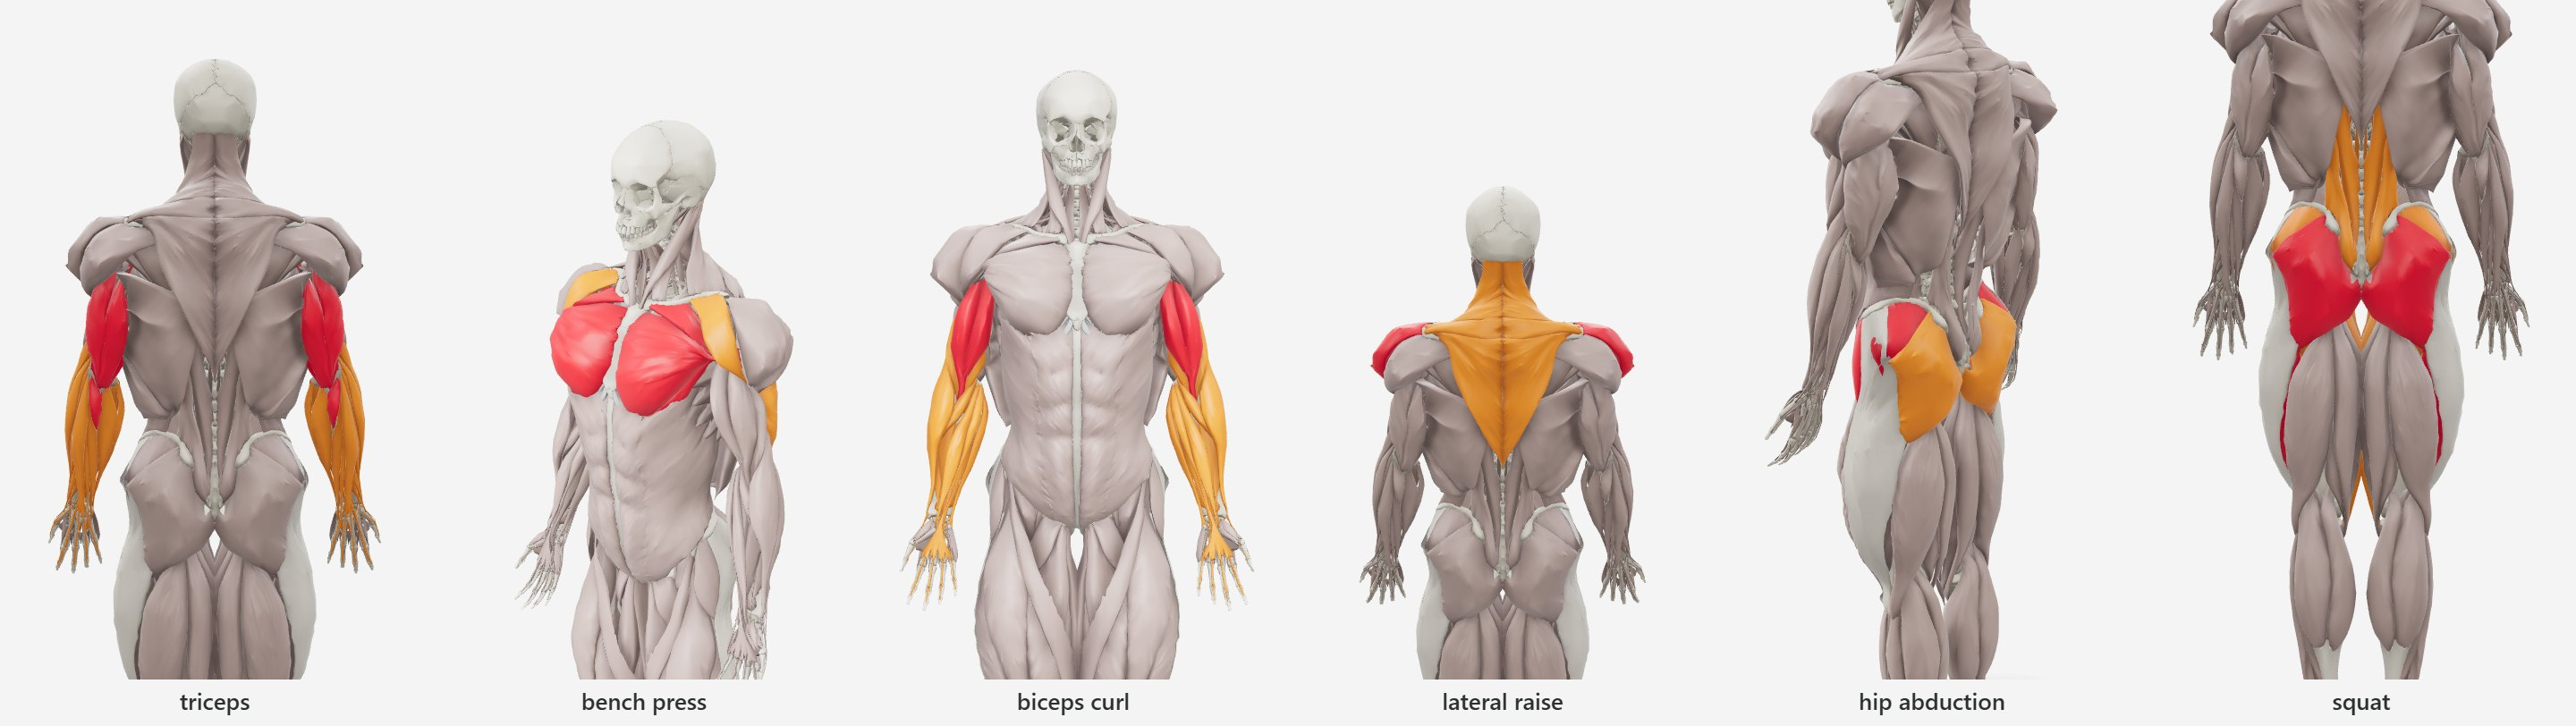
\includegraphics[width=\textwidth]{best-view.jpg}
\caption{Automatic views. The squat (right) drives quadriceps and glutes equally from opposite faces;
any single view hides half, which the split view addresses.}
\label{fig:bestview}
\end{figure*}

Applied to the 372 exercises of a training catalog (primary muscles at 100\,\%, secondary at
45\,\%), the method chose the back for 202, the front for 138, a front 3/4 view for 27, a back 3/4
view for 3 and a side view for 2 (decline presses), zooming in for 357 (Fig.~\ref{fig:bestview}).
These views were reviewed visually by the author only; a study with coaches is prepared
(Section~\ref{sec:limits}). Views are stable but not invariant across model versions: computed
on the body before the ANSUR~II calibration, 345 of the 372 had the same azimuth, most others
flipping between the two mirror-image front 3/4 views, which score almost equally on a nearly
symmetric body. When key muscles lie on opposite faces, a \emph{split view} renders the
diametrically opposite camera in the other half of the canvas, synchronized so both halves always
show opposite sides.

\section{Fitting the body to tape measures}\label{sec:fit}

\begin{table*}[t]
\centering\footnotesize
\setlength{\tabcolsep}{3.6pt}
\caption{RMS error (cm) predicting a hidden tape on 600 unseen people per sex. Mean: the
calibration half's sex mean. Then three information sets --- height, weight and body fat (h,w,f);
plus one neighbouring tape (+1); plus every other tape (all) --- each predicted by a ridge regression
trained on the calibration half (R) and by the fit (F). $^\dagger$The Navy body fat reads the neck
(and the hips for women), so the h,w,f columns are not blind for those sites.}
\label{tab:holdout}
\begin{tabular}{@{}lrrrrrrr@{\hspace{14pt}}rrrrrrr@{}}
\toprule
 & \multicolumn{7}{c}{Men} & \multicolumn{7}{c}{Women}\\
\cmidrule(lr){2-8}\cmidrule(l){9-15}
 & & \multicolumn{2}{c}{h,w,f} & \multicolumn{2}{c}{+1} & \multicolumn{2}{c}{all}
 & & \multicolumn{2}{c}{h,w,f} & \multicolumn{2}{c}{+1} & \multicolumn{2}{c}{all}\\
\cmidrule(lr){3-4}\cmidrule(lr){5-6}\cmidrule(lr){7-8}\cmidrule(lr){10-11}\cmidrule(lr){12-13}\cmidrule(l){14-15}
Site & mean & R & F & R & F & R & F & mean & R & F & R & F & R & F\\
\midrule
Biceps   & 3.45 & 1.65 & 1.60 & 1.33 & 1.36 & 1.26 & 1.51 & 2.88 & 1.33 & 1.42 & 1.17 & 1.28 & 1.18 & 1.33\\
Forearm  & 2.16 & 1.10 & 1.09 & 0.89 & 0.92 & 0.86 & 0.87 & 1.75 & 0.94 & 0.93 & 0.83 & 0.88 & 0.79 & 0.84\\
Thigh    & 5.96 & 2.30 & 2.60 & 2.26 & 2.54 & 1.59 & 2.46 & 5.61 & 2.21 & 2.52 & 2.13 & 2.43 & 1.76 & 2.33\\
Calf     & 3.06 & 1.66 & 1.66 & 1.64 & 1.61 & 1.55 & 1.58 & 2.88 & 1.65 & 1.67 & 1.59 & 1.66 & 1.46 & 1.53\\
\textit{Limb mean} & \textit{3.66} & \textit{1.68} & \textit{1.74} & \textit{1.53} & \textit{1.61} & \textit{1.31} & \textit{1.61}
 & \textit{3.28} & \textit{1.53} & \textit{1.64} & \textit{1.43} & \textit{1.57} & \textit{1.30} & \textit{1.51}\\
Neck$^\dagger$ & 2.63 & 1.39 & 1.37 & 1.37 & 1.45 & 1.23 & 1.50 & 1.83 & 1.19 & 1.19 & 1.14 & 1.22 & 1.06 & 1.13\\
Shoulders & 6.44 & 3.18 & 3.09 & 2.91 & 3.05 & 2.87 & 3.05 & 5.04 & 2.92 & 2.89 & --- & --- & 2.72 & 2.92\\
Chest    & 8.69 & 3.34 & 4.55 & 3.06 & 4.23 & 2.65 & 4.43 & \multicolumn{7}{c}{(not used)}\\
Hips     & 7.77 & 2.55 & 2.85 & 1.99 & 2.20 & 1.95 & 2.26 & 7.42 & 2.12$^\dagger$ & 2.62$^\dagger$ & 1.78 & 2.16 & 1.79 & 2.36\\
\bottomrule
\end{tabular}
\end{table*}


\paragraph{Observation model.}
For each of 12 tape sites (arm flexed, forearm, thigh, calf on both sides; neck, shoulders, chest,
hips), the pipeline stores cross-sections perpendicular to the limb axis --- or horizontal on the
trunk --- at several levels. A tape bridges concavities, so the girth is the perimeter of the convex
hull of the section, at the thickest level for limbs and the thinnest for the neck. Re-slicing the
mesh in the browser is too slow; instead each section stores \emph{material points}, the crossings
of mesh edges with the plane in a reference shape, with their per-region displacements:
$\vect q_j(\vect w)=\vect b_j+\sum_r w_r\vect d_{rj}$. The girth $G_s(\vect w)$ is the hull perimeter
(Andrew's monotone chain~\cite{andrew1979hull}); since the hull's vertex set is locally constant, its
gradient is analytic,
\begin{equation}
\frac{\partial G_s}{\partial w_r}=\sum_{(i,j)\in\text{hull}}\frac{(\vect q_j-\vect q_i)^{\!\top}}{\|\vect q_j-\vect q_i\|}\,(\vect d_{rj}-\vect d_{ri}).
\end{equation}
The signed volume of a closed mesh, $\frac16\sum_t \vect a\cdot(\vect b\times\vect c)$, is with affine
vertices an \emph{exact cubic polynomial} in $\vect w$; the GLB stores its $\approx 500$ monomials.

A tape wraps skin and subcutaneous fat. For a ring of thickness $t$ around a convex section the
perimeter grows by $2\pi t$ (Steiner), so with skinfold $S\approx 2t$ the muscle-and-bone girth is
$C-\pi S$~\cite{heymsfield1982arm,lee2000anthropometric}. Without skinfolds, the skinfold of a site
is estimated from total fat mass FM and body surface area~\cite{mosteller1987bsa}:
\begin{equation}
S = 2.5\,\text{mm} + a(\text{site},\text{sex})\left(\mathrm{FM}/\mathrm{BSA}\right)^{0.9},
\end{equation}
with coefficients reproducing the mean skinfolds of Lee et al.~\cite{lee2000anthropometric} within
3\,mm and a 20\,\% individual variation entering each measure's uncertainty --- independently per
site, a simplification the evaluation shows to be costly. Girths are carried to the model's height
through the ratio of lean masses at the normalized FFMI, divided by the height ratio (areas),
square-rooted (perimeters).

\paragraph{Objective.}
The unknowns are the region weights $\vect w$ and the FFMI $F$. We minimize
\begin{equation}
\begin{split}
E(\vect w,F)={}&\sum_s \rho_H\!\Big(\frac{G_s(\vect w)-y_s}{\sigma_s}\Big)
+\tfrac12\,\boldsymbol\Delta^{\!\top}\Sigma^{-1}\boldsymbol\Delta\\
&+\tfrac12\Big(\frac{V(\vect w)-V^\star(F)}{0.01\,V^\star(F)}\Big)^{2}
+\tfrac12\Big(\frac{F-F_0}{\sigma_F}\Big)^{2},
\end{split}
\end{equation}
with $\boldsymbol\Delta=\vect w-\boldsymbol\mu(F)$, where $y_s$ is the corrected, height-scaled tape; $\sigma_s$ combines tape technique (1\,\%), level
placement (1.2--4\,\%) and the fat estimate; $\rho_H$ is the Huber loss~\cite{huber1964robust}
($k=2.5$); $\boldsymbol\mu(F)$ and $\Sigma$ are the typical body of FFMI $F$ and the between-region
covariance; $V^\star(F)$ the muscle volume of the typical body; and $F_0,\sigma_F$ the FFMI from weight,
height and body fat with the uncertainty of the body-fat method (or the population mean with a wide
deviation when no body fat is known; the US Navy formula~\cite{hodgdon1984navy} is used when girths
allow it). The volume term is what makes a thigh larger than expected take muscle from the other
regions when the FFMI is well measured, and raise the FFMI when it is not. Trunk girths also reflect
skeletal breadth and fat distribution, which the model does not vary; they enter as a ratio over the
population mean at the same FFMI, applied to the typical body's section. We solve with
Levenberg--Marquardt~\cite{levenberg1944,marquardt1963} with an active set at the weight bounds
$[-0.15,1.35]$, iteratively reweighting the Huber terms; it converges in 3--6 iterations. The inverse
normal matrix at the optimum gives per-region uncertainties. A tape is flagged as an outlier and
removed when it deviates by more than six \emph{population} standard deviations from the prediction of
a fit without it.

\paragraph{Calibration on ANSUR~II.}
For each of the 4\,082 men and 1\,986 women of ANSUR~II~\cite{gordon2014ansur} we compute the Navy
body fat, the normalized FFMI (men $21.7\pm1.9$, women $17.7\pm1.0$) and every tape in model space as
the fit does. Per site we fit the cross-section area (girth$^2$) linearly in $F$; the typical body
$\boldsymbol\mu(F)$ reproduces these curves on the limbs and keeps the model's hypertrophy on the
trunk. ANSUR~II measures the limbs on one side only, so both sides are tied, with an \emph{assumed}
between-side deviation of 2\,\% of the girth. The covariance of the deviations at equal FFMI, minus
the modelled noise of tapes and estimated fat (at most 80\,\% of the observed variance) and projected
to the nearest positive-definite matrix, is carried to region weights through the Jacobian. In the
fit it is scaled by a factor of 3 in standard deviation, a design choice for training populations,
which we expect to vary more than soldiers (Section~\ref{sec:eval}); the correlations, which
propagate information from measured to unmeasured regions, are kept. Calibration replaced
appearance-tuned proportions: at $F=26$ the arm had carried 51\,cm of muscle alone, more than a
natural bodybuilder's flexed tape.

\begin{figure}[t]
\centering
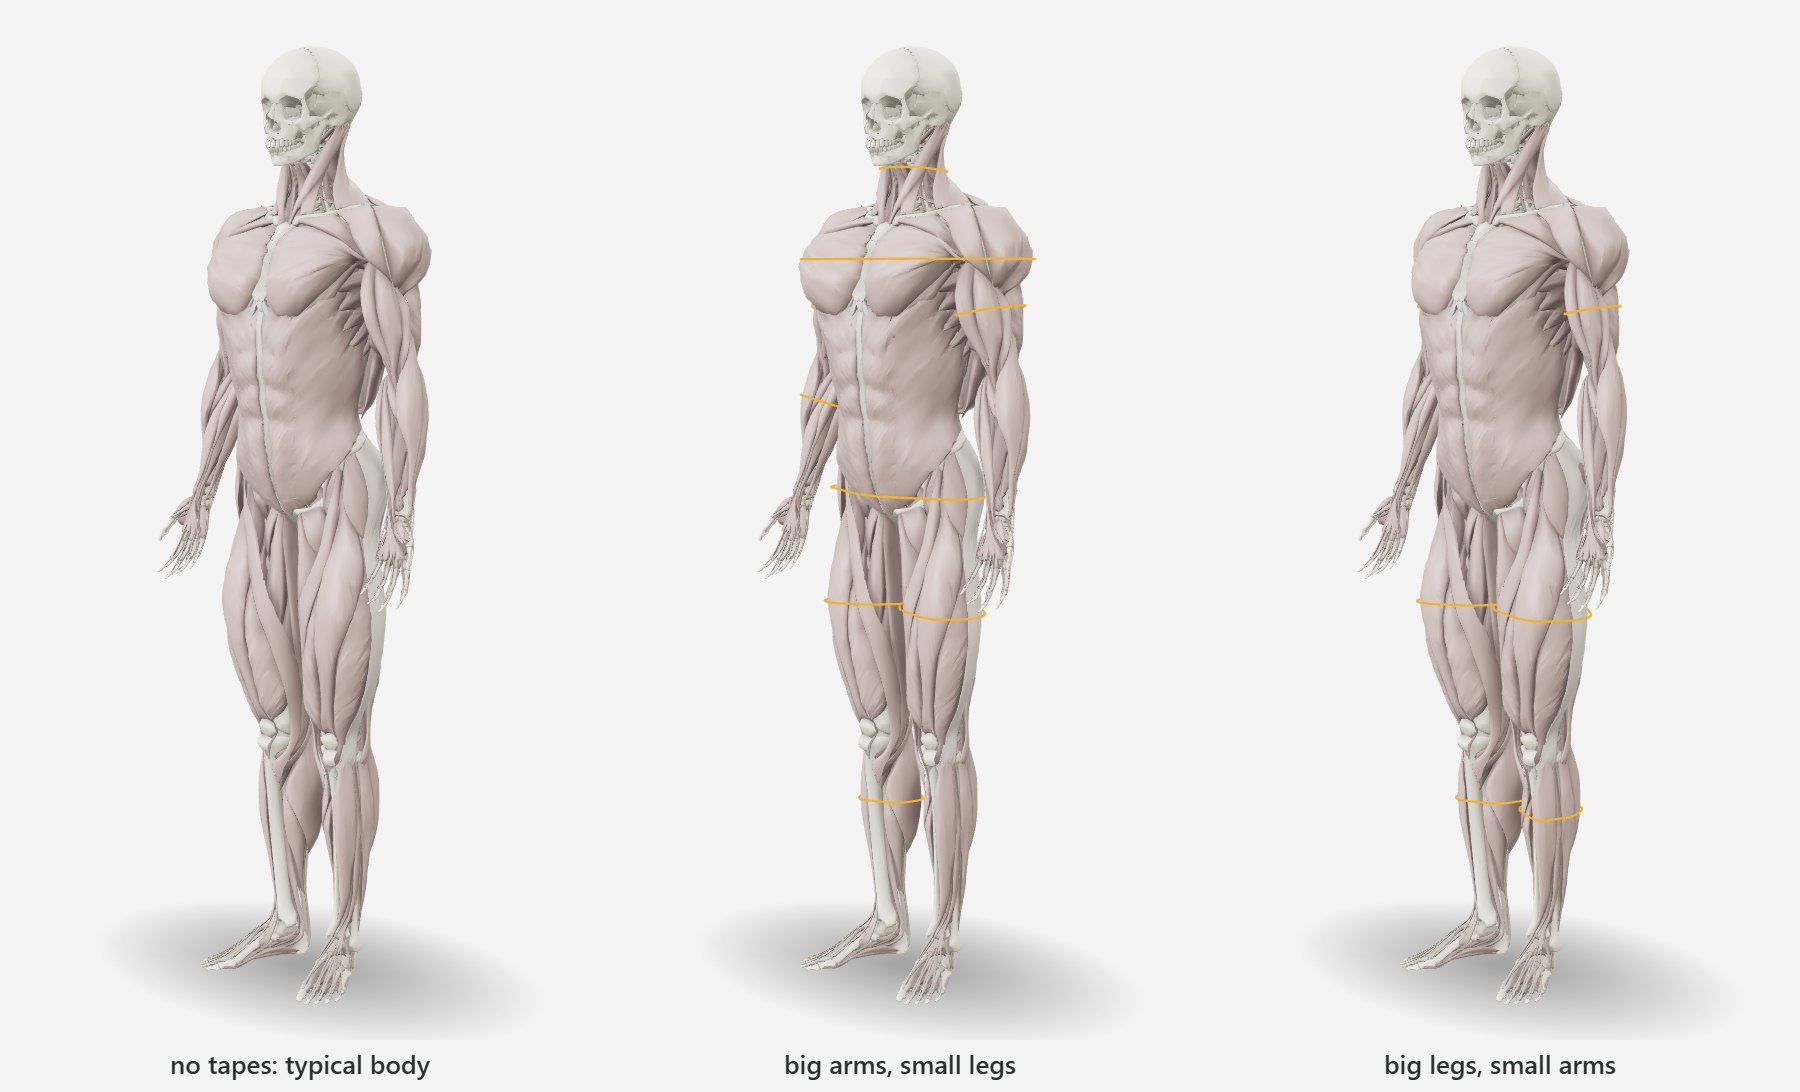
\includegraphics[width=\columnwidth]{tape-fit.jpg}
\caption{One person (178\,cm, 84\,kg, 14\,\% body fat). Left: no tapes, the typical body of the FFMI.
Centre and right: the same FFMI with large arms or large legs; muscle moves between regions and the
rings show the fitted tapes, including the estimated fat.}
\label{fig:fit}
\end{figure}

\section{Evaluation}\label{sec:eval}

\begin{table}[t]
\centering\small
\caption{Runtime cost (ms, medians). GPU: RTX 4060 Ti; CPU: SwiftShader software rasterization.}
\label{tab:perf}
\begin{tabular}{@{}lrrrr@{}}
\toprule
 & \multicolumn{2}{c}{GPU} & \multicolumn{2}{c}{CPU}\\
\cmidrule(lr){2-3}\cmidrule(l){4-5}
 & full & lite & full & lite\\
\midrule
Frame          & 2.3 & 1.3 & 256 & 156\\
Split-view frame & 3.5 & 2.0 & --- & ---\\
Pick           & 1.1 & 0.8 & 26 & 12\\
Best view      & 23  & 15  & 589 & 268\\
Tape fit (8 tapes) & 6.5 & 9.2 & --- & ---\\
\bottomrule
\end{tabular}
\end{table}

\paragraph{Geometric fidelity.}
Sampling region weights across the plausible range, the probe girths match true cross-sections of
the deformed meshes within 0.4\,\% (arms), 0.2\,\% (forearms, calves), 1.0\,\% (neck), 1.6\,\%
(shoulders), 2.0\,\% (hips) and 2.9\,\% (thighs); the volume polynomial matches the mesh to
$10^{-6}$ relative; the region morphs sum to the uniform morph to float rounding.

\paragraph{Anatomical plausibility.}
The fit constrains hull perimeters and total volume, never the inside. As a coarse check we compare
the right quadriceps of the typical body, computed from the exported meshes, with MRI volumes of 52
untrained and 16 long-term resistance-trained young men~\cite{madenwilkinson2020strong}
(Table~\ref{tab:mri}). That study reports no body composition, so we sweep a plausible body fat;
a person's quadriceps is the typical body's at their FFMI, scaled by their lean mass. The group
volume falls within $-0.6$ to $+1.4$ standard deviations of the measured means, but the model
underestimates the difference between the groups ($+37$ to $+39$\,\% for the same body-fat gap,
$+57$\,\% measured): trained men carry more quadriceps than the typical body of their FFMI. The
split between heads disagrees, at every FFMI: BodyParts3D's rectus femoris is a quarter of the
quadriceps and its vastus intermedius less than a fifth, against 13\,\% and 30\,\% by MRI. Volumes
are plausible per muscle group --- what the viewer colours --- not per head.

\begin{table}[t]
\centering\small
\setlength{\tabcolsep}{4pt}
\caption{Right quadriceps volume (cm$^3$): MRI of 52 untrained (176\,cm, 73\,kg) and 16 trained men
(183\,cm, 91\,kg)~\cite{madenwilkinson2020strong}, mean $\pm$ SD, and the model over an assumed body fat.
Last row: share of each head (vastus lateralis, intermedius, medialis; rectus femoris).}
\label{tab:mri}
\begin{tabular}{@{}lrrr@{}}
\toprule
 & MRI & Model & Body fat\\
\midrule
Untrained & $1838\pm263$ & 1943--2216 & 20--12\,\%\\
Trained & $2882\pm308$ & 2704--3041 & 16--8\,\%\\
\midrule
Heads, \% & 33\,/\,30\,/\,24\,/\,13 & 37\,/\,18\,/\,20\,/\,25 & \\
\bottomrule
\end{tabular}
\end{table}

\paragraph{Out-of-sample accuracy.}
ANSUR~II has no reference body composition, so each person's body fat is estimated --- by default
with the US Navy formula on their own neck, waist and (women) hips. Body composition is therefore a
proxy throughout, and the agreement between fitted and input FFMI below is not an independent check.
We calibrated on the even-numbered rows of the public file (2\,041 men, 993 women) and tested on the
first 600 odd-numbered rows of each sex, with no further selection. Each tape, hidden in turn, is
predicted from height, weight and body fat alone (the typical body), with one neighbouring tape, and
with all the others, and compared with two baselines trained on the calibration half on exactly the
same inputs: the sex mean and a ridge regression~\cite{hoerl1970ridge} with a cross-validated penalty
(Table~\ref{tab:holdout}).

The typical body of an FFMI halves the error of the mean and is within 0.1\,cm of the regression on
the limbs given the same three numbers (limb mean 1.74 against 1.68\,cm for men). With more tapes the
regression pulls ahead: given every other tape it is better by 0.2--0.3\,cm on the limbs, 0.9\,cm on
the men's thigh and 1.8\,cm on the chest. Explaining every tape with one anatomical body costs
accuracy once many tapes are given. A diagnostic run locates the cost: the regression's thigh error
drops from 2.24 to 1.59\,cm when the trunk tapes are added --- a large hip girth predicts a large
thigh through shared fat and pelvic breadth --- while the fit, whose prior holds only the covariance
of \emph{muscle} between regions and whose per-site fat deviations are independent, barely uses
them (2.52 to 2.46\,cm). The same mechanism explains why more tapes sometimes hurt the fit (one
neighbouring tape beats all of them for the men's biceps, neck, chest and hips): the men's biceps is
predicted to 1.33\,cm from the other limb tapes and to 1.51\,cm once the trunk tapes are added. Trunk
tapes enter as ratios and carry mostly fat and skeletal breadth; with a wide prior the fit moves trunk
regions to match them and the muscle correlations drag the limbs along. A regression, which weighs
each input by its predictive value, never loses from more inputs. Biases stay below 0.4\,cm, no real
body was flagged as an outlier, and the fitted FFMI stays within $\pm0.75$ of the input for 90\,\% of
people. Fits take 7--15\,ms on average in Node.js (Intel i7-12700F), varying between runs.

With a girth-free body fat --- Deurenberg's formula on BMI and age~\cite{deurenberg1991bmi} --- the
typical-body column becomes blind to every tape: its limb error rises to 1.88\,cm (men) and 1.69\,cm
(women), still half the mean's, and biases appear, because BMI attributes muscle to fat in muscular
soldiers (the fit raises their FFMI by 0.34 on average to reconcile the tapes).

\paragraph{Asymmetry.}
\begin{table}[t]
\centering\small
\caption{Share of a synthetic left--right difference (left tape $=$ right $\times(1+\delta)$) that the
fitted body reproduces; constant within 0.02 for $\delta=2$, 5 and 10\,\%. 300 people per sex.}
\label{tab:asym}
\begin{tabular}{@{}lrrrr@{}}
\toprule
 & Arm & Forearm & Thigh & Calf\\
\midrule
Men   & 0.81 & 0.82 & 0.81 & 0.85\\
Women & 0.50 & 0.60 & 0.49 & 0.66\\
\bottomrule
\end{tabular}
\end{table}
ANSUR~II measures one side, so real left--right differences cannot be validated on it. Imposing a
synthetic difference instead (Table~\ref{tab:asym}), the fitted body reproduces 80--85\,\% of it for
men and 48--66\,\% for women; the rest is absorbed by the prior that ties the sides and, through the
volume term, by the measured side, which moves by up to 0.35\,cm. Women's tapes carry more
uncertainty (more estimated fat), so the prior weighs more: about half of a real difference would be
drawn. How large real differences are, and whether the fit follows them, is open.

\paragraph{Width of the prior.}
Scaling the population covariance by 1, 2 or 3 in standard deviation changes every predicted tape by at
most 0.2\,cm on ANSUR~II (limb mean with all tapes: 1.60, 1.53, 1.61\,cm for men; 1.53, 1.51,
1.51\,cm for women); a factor of 2 is marginally best within this homogeneous population, and the
narrower prior removes the drag of the trunk tapes on the men's biceps (1.33 and 1.35\,cm with all
tapes at factors 1 and 2). We keep 3 as
a design choice for training populations; the only evidence is anecdotal (with factor 1, a real
thigh 15\,\% above typical was flagged as an outlier during development). For women the modelled
noise accounts for nearly all the observed between-person variance at most sites, so their covariance
sits at its floor and some correlations saturate (thigh--hips); skinfold measurements would separate
fat from muscle.

\paragraph{Performance.}
Table~\ref{tab:perf} reports medians on an NVIDIA RTX~4060~Ti (Chrome, ANGLE/Direct3D~11) and, as a
pessimistic bound, with CPU rasterization (SwiftShader, Intel i7-12700F). An idle viewer renders
nothing.

\paragraph{Reproducibility.}
Refactoring the whole code base for release (version 0.2) was verified end to end: the rebuilt models
have byte-identical binary chunks, the calibration reproduces bit for bit, all 377 activation names of
the previous version resolve to the same targets, and 17 rendering scenarios --- poses, split view,
automatic views, shapes, tape rings --- match pixel for pixel under deterministic software
rendering. Every number in this section comes from a script in the repository.

\section{Limitations and future work}\label{sec:limits}

\paragraph{Model.} The model is one male body: female proportions are skeletal transforms and every
person shares one skeleton scaled to two heights. Regions thicken as a whole --- the biceps cannot
grow apart from the triceps --- and a tape informs its entire region. The trunk is matched as a ratio
over the typical body, so skeletal breadth is not personalized. The isotropic limbs trade volume
fidelity per level for round sections, and the quadriceps heads keep the source's proportions. The
model shows no fat or skin, and the head lacks facial and masticatory muscles, which BodyParts3D
does not contain.

\paragraph{Evaluation.} Body composition was a proxy estimated from tapes or BMI, never a reference
method. The calibration population is U.S. Army personnel aged 17--58; beyond FFMI 28 (men) and 21
(women) the curves extrapolate, and at the top of the range the quadriceps look bulbous
(Fig.~\ref{fig:ffmi}). Three questions need people, and we release protocols and analysis scripts
for each: whether the fit follows \emph{real} left--right differences (both sides of every limb
measured on 20--40 adults); whether the prior, and its factor of 3, suit a \emph{trained} population
(30 or more lifters with bioimpedance or DXA, analysed for spreads 1--3); and whether coaches agree
with the automatic views (3--5 raters choose the best of eight rendered azimuths for 30 exercises,
analysed with Fleiss' $\kappa$~\cite{fleiss1971kappa} and the algorithm's agreement with the raters
compared with theirs among themselves).

\paragraph{Future work.} A covariance of the per-site fat residuals, learnt on ANSUR~II like the
muscle covariance, would let the fit use what the regression exploits; skinfold input would separate
fat from muscle directly. Per-muscle morphs, a translucent fat layer from the fitted fat, exercise
animation with the existing rig, EMG-derived activation intensities and measurements on mobile GPUs
are further steps.

\section{Conclusion}

body3d shows that an anatomically detailed, personalized muscle viewer fits the constraints of
ordinary web pages. Linearity is the thread through the design: the layered hypertrophy splits into
exactly additive regional morph targets; probes and a volume polynomial make the tape fit a small,
smooth least-squares problem; and a population prior learnt from anthropometric data lets a few tape
measures shape the whole body while conserving its muscle mass. The evaluation also measures the
price of that consistency: given many tapes, a plain regression predicts a hidden girth better,
because the model explains every tape with muscle alone. The code is released under the MIT licence
and the models under CC~BY~4.0.

\paragraph{Availability.}
{\raggedright Source, models, documentation (API, architecture, pipeline, design decisions, validation) and the
scripts reproducing every number in this paper are in the body3d repository:
\code{dev/validate-ansur.mjs} (Table~\ref{tab:holdout}), \code{dev/asymmetry-ansur.mjs}
(Table~\ref{tab:asym}), \code{dev/muscle-volumes.mjs} (Table~\ref{tab:mri}),
\code{pipeline/check\_isotropy.py} and \code{pipeline/check\_fit.py} (geometry), and the study kits
\code{dev/validate-measured.mjs} and \code{dev/view-study.mjs}.\par}

\paragraph{Acknowledgments.}
The models derive from BodyParts3D, \textcopyright{} The Database Center for Life Science, licensed
under CC Attribution 4.0 International. The calibration uses the public ANSUR~II data of the U.S.
Army. body3d was first developed for the Trace training tracker, whose exercise catalog provided the
training vocabulary and the views evaluated here.

\small
\bibliographystyle{plainnat}
\bibliography{references}

\end{document}
